\documentclass[11pt,a4paper]{article}
\usepackage[margin=0.88in,top=0.78in,bottom=0.8in,headheight=15pt]{geometry}
\usepackage[T1]{fontenc}
\usepackage{lmodern,microtype,graphicx,booktabs,array,tabularx,amsmath,amssymb}
\usepackage{caption,subcaption,float,placeins,xcolor,setspace,enumitem,fancyhdr}
\usepackage{hyperref}
\usepackage{titlesec}
\definecolor{ink}{HTML}{173E50}
\definecolor{accent}{HTML}{166781}
\definecolor{rust}{HTML}{B35D3D}
\hypersetup{colorlinks=true,linkcolor=ink,citecolor=ink,urlcolor=accent,
 pdftitle={Food Inflation and the Phillips Relationship in India},
 pdfauthor={K Harshavardhan and Pasula Kohith}}
\urlstyle{same}
\graphicspath{{assets/}}
\setstretch{1.25}
\setlength{\parindent}{0pt}
\setlength{\parskip}{5.5pt}
\setlength{\tabcolsep}{5.5pt}
\setlength{\emergencystretch}{0.6em}
\widowpenalty=10000
\clubpenalty=10000
\raggedbottom
\renewcommand{\arraystretch}{1.16}
\captionsetup{font=small,labelfont=bf,skip=5pt}
\setlist[itemize]{leftmargin=1.4em,itemsep=3pt,topsep=4pt}
\titleformat{\section}{\Large\bfseries\color{ink}}{\thesection}{0.6em}{}
\titleformat{\subsection}{\large\bfseries\color{ink}}{\thesubsection}{0.6em}{}
\titlespacing*{\section}{0pt}{16pt}{7pt}
\titlespacing*{\subsection}{0pt}{10pt}{4pt}
\pagestyle{fancy}
\fancyhf{}
\fancyhead[L]{\small\color{ink}Food inflation and unemployment}
\fancyhead[R]{\small HS455\enspace|\enspace Review draft}
\fancyfoot[C]{\small\thepage}
\renewcommand{\headrulewidth}{0.35pt}
\newcommand{\tabnote}[1]{\par\vspace{2pt}{\footnotesize\emph{Note:} #1\par}}
\newcommand{\source}[1]{{\footnotesize\emph{Source:} #1\par}}
% Edit this file to update the cover without changing the report.
\newcommand{\ReportTitle}{Food Inflation and the\\Phillips Relationship in India}
\newcommand{\ReportSubtitle}{Urban Unemployment, Core Inflation\\and the Food Contribution to Headline Variability}
\newcommand{\CourseCode}{HS455}
\newcommand{\InstructorNames}{Dr. Smruti Ranjan Behera\\Samaresh Bardhan\\Bhavesh Garg}
\newcommand{\ReportDate}{November 2026}
\newcommand{\StudentRows}{K Harshavardhan & 2023MCB1216\\Pasula Kohith & 2023EEB1232\\}


\begin{document}
\hypersetup{pageanchor=false}
\begin{titlepage}
\thispagestyle{empty}
\begin{center}
\vspace*{0.25cm}
{\fontsize{25}{31}\selectfont\bfseries\color{ink}\ReportTitle\par}
\vspace{0.5cm}
{\large\ReportSubtitle\par}
\vspace{0.8cm}
{\large\itshape A Project Report Submitted for the Course\par}
\vspace{0.2cm}
{\LARGE\bfseries\CourseCode\par}
\vspace{0.45cm}
{\normalsize\itshape Instructors\par}
\vspace{0.12cm}
{\large\InstructorNames\par}
\vfill

\includegraphics[height=4.1cm,keepaspectratio]{iit_ropar_logo.png}\par
\vspace{0.4cm}
{\Large\bfseries INDIAN INSTITUTE OF TECHNOLOGY ROPAR\par}
\vspace{0.2cm}
{\large\ReportDate\par}
\vfill
{\large\itshape Submitted by\par}
\vspace{0.3cm}
\begin{tabular}{ll}
\toprule
\textbf{Name} & \textbf{Entry number}\\
\midrule
\StudentRows
\bottomrule
\end{tabular}
\vspace{0.6cm}

{\footnotesize\color{rust}AI-assisted review draft. Student review and revision are required before submission.}
\end{center}
\end{titlepage}
\setcounter{page}{1}
\hypersetup{pageanchor=true}

% MAIN_TEXT_START
\section{Background and Motivation}

A rise in grocery bills and a rise in economy-wide demand can both push inflation up, but their links to employment can be very different. Strong demand may allow firms to raise prices while hiring more workers. A poor harvest can raise food prices even when demand and employment are weak. A single headline inflation number combines these movements. Understanding its composition is therefore a useful first step before relating inflation to unemployment.

The Phillips-curve idea suggests a negative short-run relationship between inflation and unemployment, holding other influences constant. When labour markets tighten, wage and demand pressures may increase. However, an observed correlation also reflects supply shocks, expectations and policy responses. Removing volatile food prices might make the demand-related part of inflation easier to see. This is a hypothesis to examine with data, rather than a property that core inflation must possess.

India provides a useful setting for this comparison. Food and beverages have a weight of 45.86\% in the 2012-base Combined Consumer Price Index (CPI), which covers rural and urban households. The Urban weight is lower, at 36.29\%. These are expenditure weights: they describe the basket's composition, not the proportion of inflation variability explained by food. A component can contribute much more to variability than its weight suggests if its prices move sharply or move together with other prices.

Existing research helps distinguish the questions. Behera, Wahi and Kapur find that demand conditions matter for Indian state-level inflation, with a stronger response for core inflation in their framework~\cite{behera2017}. Their activity measure is an output gap, so the present unemployment exercise is not a replication. Patra, John and George study food--non-food price dynamics and report a small positive short-run association in an error-correction model~\cite{patra2024}. Mohan and co-authors examine inflation volatility, emphasising vegetable prices~\cite{mohan2026}. These studies concern related mechanisms but different quantities.

This project brings the assignment's two questions together through a transparent empirical approach. First, it compares headline and operational-core inflation against the same unemployment observations. Second, it allocates official headline-inflation variance across food and the remaining CPI groups. The earlier food--non-food work is retained as a secondary extension. Simple calculations remain central; more detailed checks establish where the conclusions are reliable and where caution is necessary.

The distinction matters for the final interpretation. Food can account for most headline variability without its exclusion producing a clearer negative unemployment relationship. The results below show precisely this combination in the available sample.

\section{Research Questions and Hypotheses}

The first question is whether the negative relationship between inflation and unemployment strengthens when food is excluded. Two requirements follow. The relationship should first be negative, and the core-inflation slope should then be more negative than the headline slope. A positive relationship with a larger correlation does not satisfy this hypothesis.

Let $\beta_H$ and $\beta_C$ denote the unemployment slopes for headline and core inflation. The expected pattern is
\begin{equation}
\beta_H<0,\qquad \beta_C<0,\qquad
\delta=\beta_C-\beta_H<0.
\label{eq:hypotheses}
\end{equation}
The report compares $\delta$ directly, using identical observations, rather than comparing the separate significance levels of two regressions. Correlations and explanatory power provide descriptive context, but do not replace this comparison.

The second question asks how much variation in headline inflation is attributable to food. The working hypothesis is that food and beverages account for a large share because of their basket weight and price variability. Here, ``attributable'' means an accounting allocation that includes covariance with other components. It does not mean the percentage caused by independently identified food shocks.

The extension asks whether monthly food inflation helps predict subsequent non-food or core inflation after allowing for persistence and calendar effects. It concerns delayed predictability. It cannot, by itself, establish transmission through wages, expectations or input costs.

\section{Data and Methodology}
\subsection{Coverage, sources and comparability}

The price data are monthly CPI index levels on the 2012 base, from January 2013 to December 2025~\cite{cpiapi}. The unemployment comparison uses All-India Urban CPI and the Periodic Labour Force Survey (PLFS): Urban Current Weekly Status (CWS), persons aged 15 years and above. The 27 matched quarters run from 2018Q2 to 2024Q4. CWS refers to activity during the preceding seven days, and unemployment is measured as a share of the labour force~\cite{plfs2024}.

Urban price and employment coverage are matched deliberately. Combining Urban unemployment with rural-plus-urban inflation would introduce a geographic mismatch. The longer Combined CPI series is used separately for the national inflation-composition question, with Urban results alongside it. Price data after the historical base change and unemployment observations from the redesigned PLFS are not appended. The PLFS design changed from January 2025, so extending the series requires a comparability assessment~\cite{plfschange}.

The Urban CPI download contains 1,092 records: seven series for each of 156 months. All months are present. Fifty-six group/general values were checked against eight separately published anchor months. The weighted Urban groups reproduce the General index within 0.08034 index points. These checks support source consistency; they do not guarantee that every underlying price quotation is error-free.

Source reconciliation was especially important for unemployment. The API reports 21.6\% for 2019Q2 and 8.1\% for 2019Q3. The published bulletins give 8.8\% and 8.3\% for persons aged 15 and above; 21.6\% belongs to the youth row~\cite{plfs2019a,plfs2019b}. The bulletin values are retained, and both discrepancies are recorded. The other 25 API observations agree with the existing bulletin transcription.

\subsection{Constructing inflation and operational core}

Headline inflation uses the official General index. Operational core excludes the Food and Beverages and Fuel and Light groups, retaining pan/tobacco, clothing/footwear, housing and miscellaneous items. Table~\ref{tab:weights} shows the weights. Their retained total is 58.13\%; the core index is the weighted sum divided by that total.

\begin{table}[htbp]
\centering\small
\caption{2012-base Urban CPI weights and the core construction}
\label{tab:weights}
\begin{tabularx}{\linewidth}{Xrrl}
\toprule
Group & Urban weight (\%) & Share of core (\%) & Treatment\\
\midrule
Food and beverages &36.29&--&Exclude\\
Pan, tobacco and intoxicants&1.36&2.34&Retain\\
Clothing and footwear&5.57&9.58&Retain\\
Housing&21.67&37.28&Retain\\
Fuel and light&5.58&--&Exclude\\
Miscellaneous&29.53&50.80&Retain\\
\bottomrule
\end{tabularx}
\source{MoSPI CPI release tables~\cite{cpirelease}; project calculations.}
\end{table}

For example, December 2024 core is calculated from the four retained indices as
\begin{equation}
C_{\mathrm{Dec24}}=
\frac{1.36(212.2)+5.57(187.8)+21.67(181.7)+29.53(182.0)}{58.13}
=183.1505.
\label{eq:core}
\end{equation}
This is a group-based measure. Vehicle fuels and precious metals remain within miscellaneous items. Core therefore does not mean complete removal of every energy-sensitive or volatile item. Housing also makes up 37.28\% of this core. Food-only exclusion and core without housing are consequently checked as alternative compositions.

For the main annual comparison, monthly levels are averaged within each quarter. Year-on-year log inflation is $100\ln(\bar I_q/\bar I_{q-4})$. For instance, the Urban headline quarterly mean rises from 183.7333 in 2023Q4 to 192.9667 in 2024Q4, giving $100\ln(192.9667/183.7333)=4.9032\%$. This differs slightly from the ordinary percentage-change formula and from averaging published monthly inflation rates.

A second measure captures shorter-run movement: seasonally adjusted quarter-on-quarter annualised log inflation, or q/q SAAR. Monthly log indices are adjusted using robust STL with a 12-month period and a seasonal window of 13. Adjusted logs are converted back to levels before averaging. The quarterly change is then $400\ln(\bar I_q^{SA}/\bar I_{q-1}^{SA})$. Showing both measures avoids making the result depend entirely on annual averaging or one seasonal-adjustment choice.

Annualisation puts a quarterly movement on an annual-rate scale; it does not forecast the next year's inflation. Year-on-year inflation is easier to relate to familiar annual rates, but neighbouring quarters share much of the same price-change history. Twenty-seven annual observations therefore contain less independent information than twenty-seven unrelated observations. Each measure has a practical advantage and a statistical cost, which is why their agreement in direction is more useful than selecting whichever produces a preferred result.

\subsection{A direct comparison of unemployment slopes}

Ordinary least squares estimates
\begin{equation}
\pi_{H,q}=\alpha_H+\beta_H U_q+e_{H,q},\qquad
\pi_{C,q}=\alpha_C+\beta_C U_q+e_{C,q}.
\label{eq:ols}
\end{equation}
Each slope is an inflation percentage-point difference associated with a one-percentage-point difference in unemployment. Regressing $D_q=\pi_{C,q}-\pi_{H,q}$ on the same intercept and unemployment series gives $\delta=\beta_C-\beta_H$. This identity is checked numerically. The model describes association; it omits expectations, supply shocks and policy responses that would be needed for a structural interpretation.

The full sample is shown alongside a fixed exclusion of 2020Q2, 2020Q3 and 2021Q2, leaving 24 quarters. These observations combine unusual labour-market conditions with pandemic-related measurement concerns. April--May 2020 CPI also includes component-specific macro-imputation~\cite{imputation}. The exclusion is a sensitivity check, not a claim that the remaining sample is free from confounding.

HC3 and calendar-based HAC uncertainty summaries are examined. HC3 allows for unequal residual variance and adjusts for leverage; HAC also allows dependence across nearby quarters. With only 27 observations, neither provides a blanket guarantee. Simulations using the actual unemployment regressor show substantial over-rejection under persistent and overlapping errors. The intervals are therefore presented as nominal sensitivity summaries, without significance stars or confirmatory claims.

\subsection{Accounting for food's contribution to variance}

This calculation uses ordinary percentage changes, so component contributions add exactly. Let $H_t$ be official headline CPI, $I_{g,t}$ a group index, and $w_g$ its basket weight expressed as a fraction. For monthly or annual lag $k$,
\begin{equation}
\pi_t=100\left(\frac{H_t}{H_{t-k}}-1\right),\qquad
c_{g,t}=100w_g\frac{I_{g,t}-I_{g,t-k}}{H_{t-k}}.
\label{eq:contributions}
\end{equation}
An explicit residual, $r_t=\pi_t-\sum_g c_{g,t}$, retains the small difference between official headline and weighted group changes. The variance share is
\begin{equation}
s_g=100\frac{\operatorname{Cov}(c_g,\pi)}{\operatorname{Var}(\pi)}.
\label{eq:variance}
\end{equation}
Including the residual makes all shares sum to 100\%. Covariance matters because food and other contributions may reinforce or offset one another. Shares can be negative or exceed 100\%; they are not restricted expenditure weights. Paired moving-block resampling checks sensitivity to serial dependence, and matched-period and pandemic-exposure exclusions check the influence of sample choice.

\clearpage
\section{Discussion of Results}
\subsection{What the time paths show}

Figure~\ref{fig:paths} shows why the unemployment comparison needs care. Unemployment reaches 20.8\% in 2020Q2, well above the usual range of the series. Its full-sample mean is 8.88\%, with a standard deviation of 2.98 percentage points. Headline and core annual inflation average 5.21\% and 4.84\%, respectively. Their standard deviations, about one percentage point each, are much closer than the general description of core as a smoother measure might suggest.

\begin{figure}[htbp]
\centering
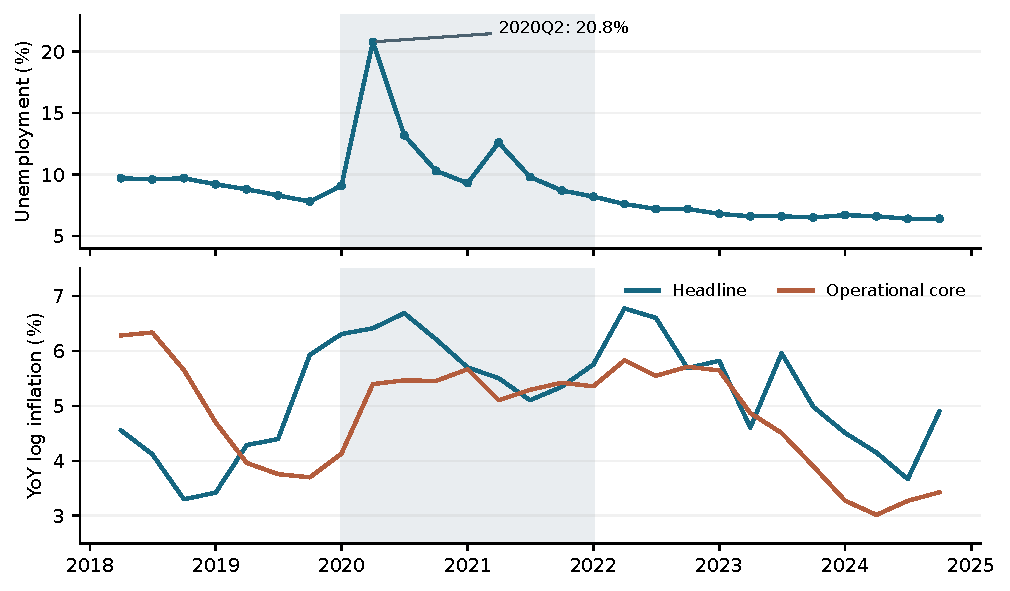
\includegraphics[width=\linewidth]{time_paths.pdf}
\caption{Urban unemployment and inflation, 2018Q2--2024Q4. Inflation is the log change of quarterly-average CPI over the same quarter a year earlier. Shading marks 2020--2021.}
\label{fig:paths}
\source{MoSPI/NSO CPI and PLFS; project calculations.}
\end{figure}

The distinction between inflation measures is useful. For q/q SAAR inflation, headline's standard deviation is 2.14 percentage points, compared with 1.23 for core. Removing food and fuel does smooth shorter-run price movement. Smoother inflation, however, does not automatically imply a stronger negative relationship with unemployment. That is a separate empirical claim.

\begin{table}[htbp]
\centering\small
\caption{Descriptive statistics for the 27 matched Urban quarters}
\label{tab:descriptive}
\begin{tabular}{lrrrr}
\toprule
Series & Mean & Median & SD & Minimum--maximum\\
\midrule
Unemployment (\%)&8.88&8.30&2.98&6.40--20.80\\
Headline YoY log inflation (\%)&5.21&5.35&1.02&3.30--6.78\\
Core YoY log inflation (\%)&4.84&5.29&0.99&3.02--6.34\\
\bottomrule
\end{tabular}
\tabnote{SD denotes the sample standard deviation. All series use identical quarter rows.}
\end{table}

\subsection{The stronger-negative-relationship hypothesis is not supported}

Table~\ref{tab:phillips} gives the direct comparison. In the full sample, the annual headline slope is $+0.094$ and the core slope is $+0.123$. Their difference is $+0.028$. The estimated pattern is positive for both measures, whereas the hypothesis requires negative slopes and a negative difference. With q/q SAAR inflation, the headline and core slopes are also positive, at $+0.059$ and $+0.222$.

\begin{table}[htbp]
\centering\small
\caption{Matched unemployment slopes and their direct difference}
\label{tab:phillips}
\begin{tabular}{llrrrr}
\toprule
Inflation & Sample & $\hat\beta_H$ & $\hat\beta_C$ & $\hat\delta$ & Nominal HC3 interval for $\delta$\\
\midrule
YoY log & Full, $n=27$ &0.094&0.123&0.028&$[-0.280,\ 0.337]$\\
YoY log & Exclusion, $n=24$ &$-0.060$&0.420&0.481&$[0.074,\ 0.888]$\\
q/q SAAR & Full, $n=27$ &0.059&0.222&0.162&$[-0.048,\ 0.373]$\\
q/q SAAR & Exclusion, $n=24$ &$-0.113$&0.321&0.434&$[-0.362,\ 1.230]$\\
\bottomrule
\end{tabular}
\tabnote{Exclusion removes 2020Q2, 2020Q3 and 2021Q2. $\delta=\beta_C-\beta_H$. Slopes are inflation percentage points per one percentage point of unemployment. Intervals are nominal 95\% sensitivity summaries; small-sample calibration is weak.}
\end{table}

The arithmetic is straightforward: $0.1228-0.0943=0.0285$ for the full annual sample. This positive difference cannot be described as a strengthening of a negative relationship. The correlation is also positive: 0.276 for headline and 0.370 for core. The larger core correlation and $R^2$ of 0.137, compared with 0.076 for headline, indicate a closer positive fit, not support for the proposed negative pattern.

After the three pandemic quarters are removed, the headline slopes become slightly negative, while core remains positive. This again fails the hypothesised pattern. The annual slope-difference interval is entirely positive under HC3, but its nominal significance should not be treated as firm evidence of a positive structural relationship. The purpose of the comparison is to show the observed direction and its sensitivity honestly.

\begin{figure}[htbp]
\centering
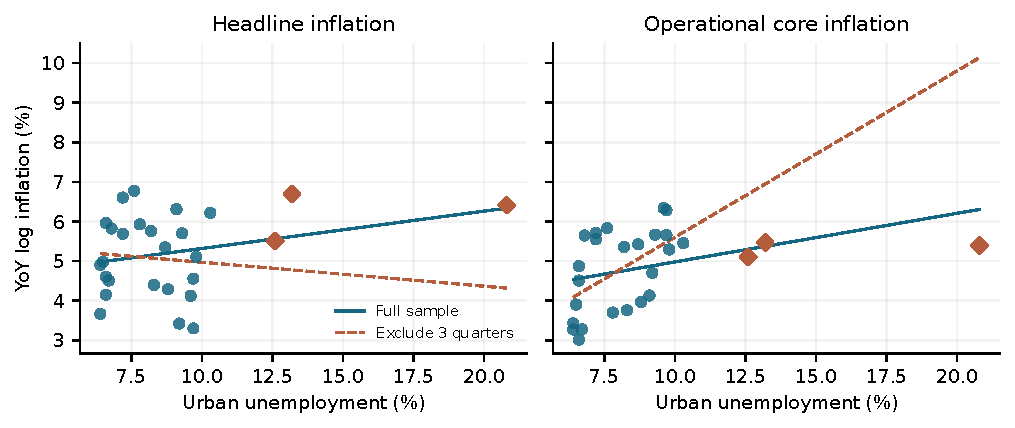
\includegraphics[width=\linewidth]{scatter_yoy.pdf}
\caption{Annual inflation and unemployment on identical rows. Blue solid lines use all 27 quarters; rust dashed lines exclude the three pandemic quarters, marked by diamonds. Dashed lines extend across the full horizontal range only to make the slope comparison visible.}
\label{fig:scatter}
\source{Project calculations; simple OLS fits.}
\end{figure}

Figure~\ref{fig:scatter} helps explain the difference between a fitted line and an economic mechanism. The observations do not trace a stable downward-sloping curve. Common shocks can affect prices and employment together, and inflation can change while unemployment is already trending down. The positive core slope should therefore be read as a feature of this period and specification. It does not establish that increasing unemployment raises inflation.

\subsection{How sensitive is that answer?}

Pandemic leverage is substantial. Measured around the full-sample unemployment mean, 2020Q2 alone contributes 61.38\% of its centred sum of squares. The three excluded quarters together contribute about 75.43\%. After exclusion, the unemployment standard deviation falls to 1.32 percentage points. Removing unusual observations reduces their influence, but also removes much of the information available for estimating a slope.

The core result is checked beyond this exclusion. Food-only exclusion keeps the full-sample slopes positive, so the finding does not depend solely on removing fuel. Removing housing from core also leaves positive slopes. Leaving out one quarter at a time preserves the positive core sign. Alternative STL windows and shorter seasonal histories give the same qualitative result for q/q inflation. Appendix~\ref{app:robustness} reports selected checks.

A calendar trend changes some slope differences, especially for annual inflation. In the full annual sample, the difference becomes negative after the trend is included, but both inflation slopes remain positive. It still fails the complete hypothesis. This illustrates why one favourable coefficient is insufficient: the signs, sample, transformation and economic interpretation must be considered together. The defensible conclusion is that strengthening is not supported by this sample, with limited power to assess a structural Phillips curve.

\subsection{Food explains most measured headline variability}

Food's covariance allocation is 88.71\% for monthly Combined headline changes and 80.96\% for year-on-year changes. The corresponding Urban allocations are 79.85\% and 64.69\% (Table~\ref{tab:variance}). Food therefore accounts for most measured variation in both geographic baskets, although the percentage is not constant across measures.

\begin{table}[htbp]
\centering\small
\caption{Food allocation to official headline-inflation variance}
\label{tab:variance}
\begin{tabular}{lrrr}
\toprule
CPI basket & Food expenditure weight (\%) & Monthly share (\%) & YoY share (\%)\\
\midrule
Combined&45.86&88.71&80.96\\
Urban&36.29&79.85&64.69\\
\bottomrule
\end{tabular}
\tabnote{Raw ordinary percentage changes. Monthly sample: February 2013--December 2025, $n=155$; YoY sample: January 2014--December 2025, $n=144$. Shares include covariance and an explicit aggregation residual.}
\end{table}

The monthly Combined calculation provides a useful example. Headline variance is 0.44393 and its covariance with the food contribution is 0.39381, both measured in squared percentage points. Equation~\eqref{eq:variance} gives $100(0.39381/0.44393)=88.71\%$. Comparing 88.71\% with the 45.86\% basket weight shows why weight alone is not an explanation of variability. The contribution's movement and its covariance with the whole basket also matter.

The Urban allocation is lower than the Combined allocation. A smaller food weight contributes to this difference, but cannot explain it on its own: group volatility and covariance also differ between the baskets. Keeping both sets of results visible avoids treating Urban employment evidence as representative of rural labour markets, while still answering the wider composition question. The comparison is about the measured baskets, not differences in individual households' exposure to price increases.

\begin{figure}[htbp]
\centering
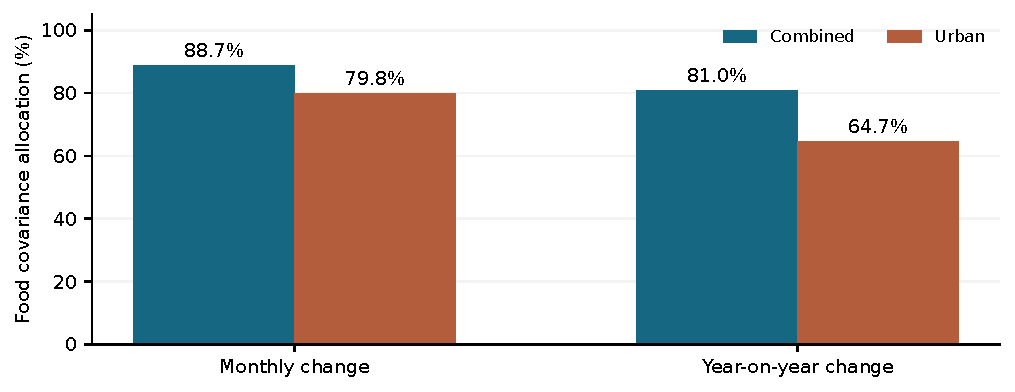
\includegraphics[width=\linewidth]{food_variance.pdf}
\caption{Food's allocation to official headline variance. The lower annual shares show that the measured allocation depends on the time horizon; the bars are accounting shares, not causal effects.}
\label{fig:variance}
\source{Official CPI levels and group weights; project calculations.}
\end{figure}

The result is reasonably stable across the checks used here. Over the matched 2018Q2--2024Q4 period, food's monthly Combined allocation is 89.07\%; excluding monthly changes exposed to the April--May 2020 imputation gives 88.62\%. Separate pre-2020 and post-2021 calculations remain food-dominated. Descriptive 12-month moving-block bounds are 85.94--93.14\% for the monthly Combined share, and 70.48--98.98\% for the annual share. The wide annual range reflects limited independent information in overlapping changes.

An earlier project figure of 90.59\% is also reproducible, but describes a reconstructed seasonally adjusted Combined aggregate. It should not replace the official-headline figures above. Adjusting headline and each group independently with STL creates a substantial seasonal-reconciliation residual, because the resulting series need not add together. Appendix~\ref{app:accounting} separates these targets. This distinction prevents a precise-looking percentage from being given a broader meaning than its construction permits.

\subsection{Extension: food--non-food predictability}

The secondary monthly model relates non-food or core inflation to three delayed food-inflation terms, current food inflation, one own lag, month effects and a pooled pandemic control. It uses 147 continuous monthly observations, October 2013--December 2025. The sum of the delayed food coefficients is $-0.0035$ for non-food and $-0.0188$ for core. Their HC3 intervals include zero and positive values (Table~\ref{tab:spillover}).

\begin{table}[htbp]
\centering\small
\caption{Secondary delayed food-inflation association}
\label{tab:spillover}
\begin{tabular}{lrrr}
\toprule
Outcome & Sum of lags 1--3 & Nominal HC3 interval & Joint bootstrap tail\\
\midrule
Non-food inflation&$-0.0035$&$[-0.0592,\ 0.0523]$&0.4361\\
Operational-core inflation&$-0.0188$&$[-0.0690,\ 0.0313]$&0.4661\\
\bottomrule
\end{tabular}
\tabnote{The joint test concerns all three delayed coefficients together; it is distinct from the interval for their sum. Restricted-null block-wild calculation: 19,999 draws, six-month blocks.}
\end{table}

The interval for the sum and the joint test answer different questions. The sum describes the combined delayed association when food inflation is higher across the three lagged months. A joint test asks whether all three delayed coefficients can be treated as zero together. Positive and negative coefficients can offset in the sum, so the two summaries need not agree. Reporting both prevents a small sum from being mistaken for evidence that every delayed response is absent. Neither summary removes the model's limited ability to detect small effects.

These estimates do not detect a positive delayed association under this model. They do not establish zero spillover. In an independent recursive simulation, an equally distributed delayed sum of 0.048 is detected in only 5.4\% of 1,000 non-food datasets under the specified persistent-error design. Moreover, the RBI's 0.048 is a short-run sum from a different ARDL specification, not our delayed-only quantity~\cite{patra2024}. Reverse predictability is specification-dependent and exploratory. Without identified shocks and reliable common-driver controls, neither direction supports a causal transmission claim.

The same caution applies to timing. A same-month food coefficient can reflect common costs or simultaneous adjustment rather than a sequence running from food to other prices. Delayed coefficients ask a narrower question, conditional on the included controls. Keeping these quantities separate helps reconcile a large food variance allocation with weak evidence of delayed predictability: the former can arise directly within headline accounting, without a strong estimated response in another price basket.

\clearpage
\section{Conclusion and Policy Implications}

The two questions lead to complementary conclusions. Food accounts for most raw official headline-inflation variability: approximately 89\% of monthly Combined variance and 81\% of annual variance in the historical sample. Yet excluding food and fuel does not produce a stronger negative unemployment relationship in the matched Urban data. Core's estimated slope is positive under both primary inflation measures, including after the fixed pandemic exclusion. Food-price volatility and Phillips-curve strength are therefore distinct empirical issues.

The scope of this conclusion is important. The unemployment comparison covers Urban persons aged 15 and above over 27 quarters. A pandemic observation accounts for a large part of unemployment variation; annual inflation overlaps across quarters; and both inflation and unemployment respond to influences omitted from a simple regression. The findings evaluate the assignment's hypothesis within this sample. They do not establish the absence of a structural Phillips curve in India or justify a numerical inflation--employment trade-off for policy.

The composition results nevertheless explain why monitoring food prices matters. Weather, market arrivals, storage and distribution conditions are relevant subjects for inflation monitoring when food accounts for such a large variance allocation. The broader policy discussion is consistent with RBI research emphasising vegetable-price variability and the risks associated with persistent food-price pressures~\cite{mohan2026,patra2024}. The present accounting cannot measure the effectiveness of particular supply interventions, and a weak estimated delayed association is not a reason to assume food shocks are harmless.

Headline and core should consequently be read together. Headline captures the prices households actually face, while core can help describe broader price pressures. Its usefulness should be assessed from its construction and behaviour rather than assumed from the label. In this study, core smooths short-run inflation but does not reveal the expected negative unemployment slope.

The analysis also sets a limit on what can be inferred from a headline number. A large food contribution does not show that domestic demand is excessive, and an estimated core slope does not provide a policy rule. Policymakers would need to distinguish temporary price movements from sustained pressures using additional evidence. Our results support that distinction while leaving the appropriate size and timing of any policy response unresolved.

Further research could examine a fully validated state panel, expectations and common cost drivers, while respecting survey changes and missing pandemic price data. For this project, the principal contribution is a clear separation of accounting, association and causation. Simple models, matched definitions and explicit validation allow a useful answer even when the expected hypothesis is not supported.
\label{main:last}
% MAIN_TEXT_END

\clearpage
\addcontentsline{toc}{section}{References}
\begin{thebibliography}{99}\small
\setlength{\itemsep}{6pt}
\bibitem{cpiapi} Ministry of Statistics and Programme Implementation (MoSPI). \emph{Consumer Price Index API}, version 2.0.0. Historical 2012-base Current Series, All India Urban. Retrieved 21 November 2026. \url{https://esankhyiki.mospi.gov.in/macroindicators?product=cpi&tab=api}. Query schema and complete raw responses are archived in the research package.
\bibitem{cpirelease} National Statistical Office (NSO) (2025). \emph{Consumer Price Index Numbers on Base 2012=100 for January 2025}. Release dated 12 February, Annexure I (December 2024 final values and group weights). \url{https://www.mospi.gov.in/sites/default/files/press_release/CPI_PR_12Feb25.pdf}.
\bibitem{plfs2024} NSO (2025). \emph{Quarterly Bulletin, Periodic Labour Force Survey, October--December 2024}. Statement 5 and age-15+ Urban tables. \url{https://mospi.gov.in/sites/default/files/publication_reports/PLFS_Quarterly_Bulletin_Oct-Dec24.pdf}. Earlier bulletin sources for each quarter are recorded in the dataset.
\bibitem{plfs2019a} NSO. \emph{Quarterly Bulletin, Periodic Labour Force Survey, April--June 2019}. Statement 5, printed p.~6 (PDF p.~9). \url{https://www.mospi.gov.in/sites/default/files/publication_reports/Quarterly_Bulletin_PLFS_April_June_2019_M_0.pdf}.
\bibitem{plfs2019b} NSO. \emph{Quarterly Bulletin, Periodic Labour Force Survey, July--September 2019}. Statement 5, printed p.~6 (PDF p.~9). \url{https://mospi.gov.in/sites/default/files/publication_reports/Quarterly_Bulletin_July_September_2019_M.pdf}.
\bibitem{plfschange} MoSPI (2025). \emph{PLFS: Changes in 2025}. Survey-design and comparability note. \url{https://www.mospi.gov.in/sites/default/files/publication_reports/PLFS_Changes-in-2025_rev.pdf}.
\bibitem{imputation} NSO (2020). \emph{Compilation of Consumer Price Index: A Technical Note}. Table 1, imputed April--May 2020 indices. \url{https://www.mospi.gov.in/sites/default/files/press_release/CPI%20Technical%20Note%20on%20Imputation.pdf}.
\bibitem{behera2017} Behera, H., Wahi, G., and Kapur, M. (2017). \emph{Phillips Curve Relationship in India: Evidence from State-Level Analysis}. RBI Working Paper Series (DEPR), 08/2017, 3 July. \url{https://rbi.org.in/Scripts/PublicationsView.aspx?id=17752}.
\bibitem{patra2024} Patra, M.~D., John, J., and George, A.~T. (2024). ``Are Food Prices the `True' Core of India's Inflation?'' \emph{RBI Bulletin}, 18 January, especially Table 3. \url{https://rbi.org.in/Scripts/BS_ViewBulletin.aspx?Id=22323}.
\bibitem{mohan2026} Mohan, R., Hasan, S., Sarkar, S., and John, J. (2026). ``Retail Inflation Volatility in India: Sources, Determinants, and Implications.'' \emph{RBI Bulletin}, 20 February. \url{https://www.rbi.org.in/Scripts/BS_ViewBulletin.aspx?Id=23980}.
\end{thebibliography}

\clearpage
\appendix
\section{Selected Robustness and Influence Checks}
\label{app:robustness}

\begin{figure}[htbp]
\centering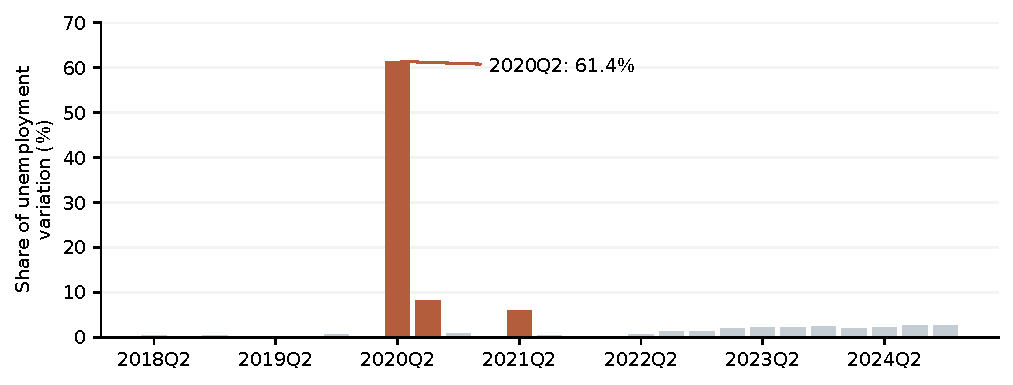
\includegraphics[width=\linewidth]{leverage.pdf}
\caption{Each quarter's share of centred unemployment variation, calculated around the full-sample mean. The three pandemic quarters together account for 75.43\%.}
\end{figure}

\begin{table}[htbp]
\centering\small
\caption{Selected slope checks: headline and alternative inflation}
\begin{tabularx}{\linewidth}{Xrrrr}
\toprule
&\multicolumn{2}{c}{YoY log}&\multicolumn{2}{c}{q/q SAAR}\\
\cmidrule(lr){2-3}\cmidrule(lr){4-5}
Check &Headline&Alternative&Headline&Alternative\\
\midrule
Full sample & 0.094 & 0.123 & 0.059 & 0.222\\
Exclude three pandemic quarters & -0.060 & 0.420 & -0.113 & 0.321\\
Exclude all of 2020--2021 & -0.318 & 0.488 & -0.325 & 0.267\\
Full sample, calendar trend & 0.149 & 0.065 & 0.099 & 0.219\\
Full sample, exclude food only & 0.094 & 0.169 & 0.059 & 0.220\\
Full sample, core without housing & 0.094 & 0.191 & 0.059 & 0.448\\
\bottomrule
\end{tabularx}
\tabnote{Alternative means operational core unless stated otherwise. Food-only exclusion retains fuel/light; core without housing excludes food, fuel/light and housing. All comparisons within a row use identical samples and controls.}
\end{table}


\begin{figure}[htbp]
\centering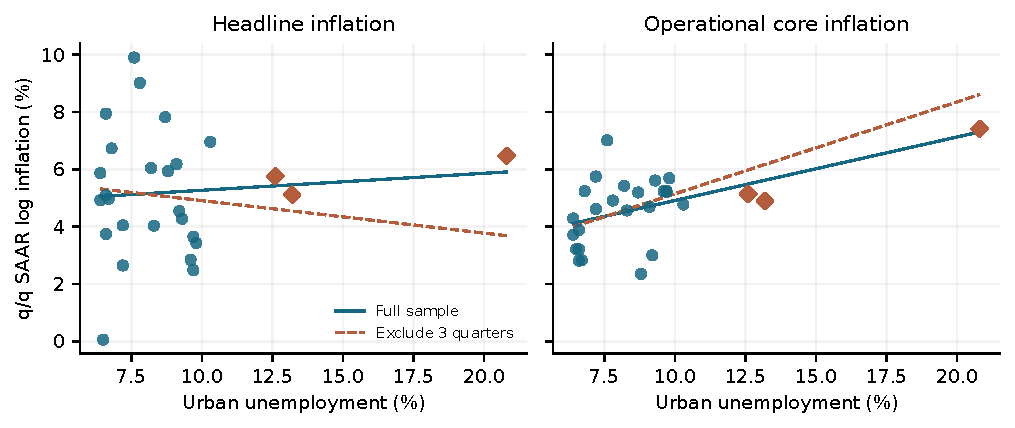
\includegraphics[width=\linewidth]{scatter_qoq.pdf}
\caption{Quarter-on-quarter seasonally adjusted annualised inflation. The same full/exclusion samples and line conventions as Figure~\ref{fig:scatter} are used.}
\end{figure}

\FloatBarrier
\section{Accounting Definitions and Validation}
\label{app:accounting}

\begin{table}[htbp]
\centering\small
\caption{Complete covariance allocation to raw official headline variance (\%)}
\begin{tabular}{llrrrr}
\toprule
Basket &Change&Food&Fuel/light&Other four groups&Residual\\
\midrule
Combined & Monthly & 88.71 & 1.45 & 8.96 & 0.88\\
Combined & YoY & 80.96 & 4.03 & 14.94 & 0.07\\
Urban & Monthly & 79.85 & 1.57 & 18.98 & -0.41\\
Urban & YoY & 64.69 & 6.83 & 28.56 & -0.08\\
\bottomrule
\end{tabular}
\tabnote{Each row sums to 100\% before rounding. ``Residual'' closes the difference between official headline and weighted-group percentage changes. A negative residual allocation is permitted. The method allocates cross-covariances; it does not assume components are independent.}
\end{table}


\subsection*{Why the seasonally adjusted figures differ}
The legacy 90.5899\% is reproduced by summing contributions from seasonally adjusted groups and dividing food covariance by the variance of that reconstructed total. By contrast, independent STL adjustment of official General and all six groups produces a reconciliation residual. Its variance allocation is 24.2410\% in Combined CPI and 25.0889\% in Urban CPI. The corresponding food shares are 69.7544\% and 61.3913\%. This residual includes the inconsistency introduced by separate seasonal adjustment; it is not an economic price category. The raw official-headline accounting is therefore the main reported answer.

\subsection*{Data checks and exclusions}
The Urban CPI input has 156 consecutive months, one value per group/general/month, the correct base and sector, and no missing index levels. Eight independently published anchor months provide 56 comparisons. April--May 2020 flags follow the technical note's group-specific annotations: Urban pan/tobacco is macro-imputed in April, but is not marked macro-imputed in May. Urban housing and fuel/light are not marked as such in either month. This does not imply absence of all elementary-level imputation.

For monthly variance sensitivity, changes using April--May 2020 in a numerator or denominator are removed; annual sensitivity removes April--May 2020 and April--May 2021. For the quarterly comparison, the fixed exclusion removes the imputation-exposed 2020Q2 and relevant q/q comparison 2020Q3, together with the second-wave quarter 2021Q2. No missing state indices are interpolated. A proposed state panel remains unvalidated future work and supplies no reported estimates.

\section{Inference, Reproducibility and Draft Disclosure}
\label{app:inference}

\begin{table}[htbp]
\centering\small
\caption{Recursive monthly-model calibration: rejection rates under a true zero delayed effect (\%)}
\begin{tabularx}{\linewidth}{lXrrr}
\toprule
Outcome &Error process&HAC(6)&HC3&Block-wild\\
\midrule
Non-food & Independent Gaussian & 13.3 & 5.1 & 4.0\\
Non-food & AR/GARCH Gaussian & 14.7 & 5.4 & 5.1\\
Non-food & AR/GARCH, heavy tails & 13.7 & 5.9 & 6.1\\
Core & Independent Gaussian & 13.4 & 5.1 & 4.3\\
Core & AR/GARCH Gaussian & 15.9 & 5.9 & 7.1\\
Core & AR/GARCH, heavy tails & 14.2 & 5.4 & 5.9\\
\bottomrule
\end{tabularx}
\tabnote{Nominal rejection rate is 5\%. Each cell uses 1,000 datasets; block-wild tests use 999 inner draws. Approximate Monte Carlo standard errors near 5\% are 0.7 percentage points. Core block-wild rejection reaches 7.1\% in one design; a bootstrap is not presumed exact.}
\end{table}

\begin{table}[htbp]
\centering\small
\caption{Illustrative power for the non-food equation under AR/GARCH errors}
\begin{tabular}{rrrr}
\toprule
True delayed sum&HAC(6) rejection (\%)&HC3 rejection (\%)&Block-wild rejection (\%)\\
\midrule
0.048 & 17.6 & 7.6 & 5.4\\
0.100 & 56.9 & 39.2 & 31.6\\
0.200 & 98.2 & 97.7 & 93.8\\
\bottomrule
\end{tabular}
\tabnote{The effect is distributed equally over three delayed coefficients. These results concern a specified synthetic process, not the true unknown data-generating process. On this grid, 80\% bootstrap power is reached between sums 0.100 and 0.200; an exact minimum detectable effect is not estimated. HAC rejection also reflects its oversized null behaviour.}
\end{table}


\subsection*{Validation of calculations}
The direct quarterly slope difference is checked against the difference of separately fitted slopes, including when a calendar trend is included. Calendar HAC uses actual quarter distances after exclusions. The original 2,000-replication aggregate-design simulation is reproduced exactly. The monthly extension additionally uses 1,000 recursive datasets per scenario and 999 inner bootstrap draws: lagged outcomes are regenerated, rather than held fixed by the data-generating process. Gaussian, persistent heteroskedastic, and heavy-tailed errors are considered. Results are design-specific, not a universal validity certificate.

All 20 historical monthly-model delayed sums and sample sizes are reproduced. Fourteen new automated tests cover source resolutions, actual regression outputs, quarterly completeness, exact variance accounting and inference behaviour. Seven targeted inference/selection defects are deliberately injected and caught. Original source/output integrity manifests remain valid. These checks establish reproducibility and software behaviour; they cannot establish causal identification.

The reported monthly primary joint probabilities use 19,999 six-month block-wild draws and model-specific seeds. Same-month tests use 49,999 draws. In the non-food equation, the same-month coefficient is 0.0377 and its bootstrap tail probability is 0.0628. Current-plus-three-lag sums are 0.0342 for non-food and 0.0180 for core, with HC3 intervals $[-0.0382,0.1067]$ and $[-0.0494,0.0854]$. These are compatible with small positive associations. Historical exclusions with compressed outcome rows are not promoted to calibrated HAC/bootstrap inference.

Reverse monthly predictability remains exploratory across five historical specifications. A further post-results relative-price sensitivity uses the historical STL reverse own-lag order zero and adds lagged $100\ln(I_{food}/I_{nonfood})$. Its 49,999-draw joint tail probability changes from 0.0965 to 0.0341. This illustrates specification dependence and does not establish cointegration or a causal direction. Multiple specifications are not treated as independent confirmations.

\subsection*{Source package and reproduction}
The companion research package contains raw API pages, bulletin sources, independent CPI anchors, processed datasets, all sensitivity tables, source reconciliations and Python scripts. Main tables and figures use saved outputs, without reselecting a specification for the report. The report source package includes the figure-generation script and a data-to-table audit. The main-text word count and page ranges are provided in the accompanying preparation notes. References and appendices are excluded from that count.

\subsection*{AI assistance and review status}
AI assistance was used for source research, programming, statistical checks, figures and preparation of this draft, including its prose. This disclosure does not certify an AI-content percentage. The named students must check the results, revise the explanation in their own words where required, and ensure that the final submission follows the course's AI-use rule. No student approval, independent human audit or compliance with the below-30\% requirement is asserted by this draft. The assignment requirements quoted in the project brief were followed; the originally named assignment PDF was unavailable for direct verification.

\end{document}
